\documentclass[aspectratio=169]{beamer}
\usepackage{fontspec}
\usefonttheme{professionalfonts}
\usepackage{amsmath,amssymb,amsthm}
\usepackage{arydshln,mathtools}
\usepackage{bm}
\usepackage{color}
\definecolor{theme}{RGB}{0,73,114}
\usepackage{multicol}
%\usepackage[caption=false]{subfig}
\usepackage{subcaption}
\usepackage{tikz-cd}


\usepackage{comment}

\usepackage{graphicx}
\usepackage{diffcoeff}
\usepackage{dsfont}
\usepackage{mathrsfs}
\usepackage[most]{tcolorbox}

\usepackage{xspace}
\usepackage{appendixnumberbeamer}


\usepackage{media9}
\usepackage[backend=bibtex, style=verbose]{biblatex}

\bibliography{biblio}
%\renewcommand\bibfont{\scriptsize}

\addtobeamertemplate{footnote}{\vspace{-6pt}\advance\hsize-0.5cm}{\vspace{6pt}}
\makeatletter
% Alternative A: footnote rule
\renewcommand*{\footnoterule}{\kern -3pt \hrule \@width 2in \kern 8.6pt}
% Alternative B: no footnote rule
% \renewcommand*{\footnoterule}{\kern 6pt}
\makeatother


\makeatletter
\g@addto@macro\normalsize{%
	\setlength\abovedisplayskip{8pt}
	\setlength\belowdisplayskip{8pt}
	\setlength\abovedisplayshortskip{8pt}
	\setlength\belowdisplayshortskip{8pt}
}
%\makeatother

\graphicspath{{./Images/}}



% Math macros
\DeclareMathOperator*{\grad}{grad}
\DeclareMathOperator*{\Grad}{Grad}
\DeclareMathOperator*{\Div}{Div}
\renewcommand{\div}{\operatorname{div}}
\DeclareMathOperator*{\Hess}{Hess}
\DeclareMathOperator*{\curl}{curl}


\DeclareMathOperator{\tr}{tr}

\DeclareMathOperator{\Dom}{Dom}
\DeclareMathOperator*{\esssup}{ess\,sup}

\newcommand{\bbR}{\mathbb{R}}
\newcommand{\bbF}{\mathbb{F}}
\newcommand{\bbA}{\mathbb{A}}
\newcommand{\bbB}{\mathbb{B}}
\newcommand{\bbV}{\mathbb{V}}
\newcommand{\bbS}{\mathbb{S}}

\newcommand{\inner}[3][]{\ensuremath{( #2, \, #3 )_{#1}}}
\newcommand{\dualpr}[3][]{\ensuremath{\langle #2 \, \vert #3 \rangle_{#1}}}

\newcommand{\bilprod}[2]{\langle \langle \, #1, #2 \, \rangle \rangle}
\newcommand*{\dual}[1]{\ensuremath{\widehat{#1}}}


\DeclareMathOperator*{\argmax}{arg\,max}
\DeclareMathOperator*{\argmin}{arg\,min}

\newtheorem{proposition}{Proposition}
\newtheorem{remark}{Remark}
\newtheorem{hypothesis}{Hypothesis}
\newtheorem{assumption}{Assumption}
\newtheorem{conjecture}{Conjecture}


\def\onedot{$\mathsurround0pt\ldotp$}
\def\cddot{% two dots stacked vertically
	\mathbin{\vcenter{\baselineskip.67ex
			\hbox{\onedot}\hbox{\onedot}}%
}}


\setbeamertemplate{blocks}[rounded][shadow]

\setbeamercolor{block body alerted}{bg=alerted text.fg!10}
\setbeamercolor{block title alerted}{bg=alerted text.fg!20}
\setbeamercolor{block body}{bg=structure!10}
\setbeamercolor{block title}{bg=structure!20}
\setbeamercolor{block body example}{bg=green!10}
\setbeamercolor{block title example}{bg=green!20}

% Remove navigation bar
\setbeamertemplate{navigation symbols}{}

\addtobeamertemplate{navigation symbols}{}{%
	\usebeamerfont{footline}%
	\usebeamercolor[fg]{footline}%
	\hspace{1em}%
	\insertframenumber/\inserttotalframenumber
}


\makeatletter \renewcommand\d[1]{\ensuremath{%
		\;\mathrm{d}#1\@ifnextchar\d{\!}{}}}
\makeatother


%% At begin of each section: show current section and all subsections in the section if any
%% At begin of each subsection except first: show only the current section/subsection
\newif\iftocsub
\tocsubtrue
\AtBeginSection[] {
	\begin{frame}[noframenumbering]{Outline}
		\tableofcontents[sectionstyle=show/shaded, subsectionstyle=show/show/hide]
	\end{frame}
	\tocsubfalse
}
\AtBeginSubsection[] {
	\iftocsub
	\begin{frame}[noframenumbering]{Outline}
		\tableofcontents[currentsubsection, sectionstyle=show/shaded, subsectionstyle=show/shaded/hide]
	\end{frame}
	\fi
	\tocsubtrue
}

\newcommand{\beginbackup}{
	\newcounter{framenumbervorappendix}
	\setcounter{framenumbervorappendix}{\value{framenumber}}
}
\newcommand{\backupend}{
	\addtocounter{framenumbervorappendix}{-\value{framenumber}}
	\addtocounter{framenumber}{\value{framenumbervorappendix}} 
}


\begin{document}
	
	
	\begin{frame}[plain]
		
		\input{Title_ExplicitPFEM}
		
	\end{frame}
	
	
	\begin{frame}{Outline}
		
		\tableofcontents
		
	\end{frame}

\section{Introduction}

\begin{frame}{Introduction}
	Given a port-Hamiltonian PDE with mixed boundary conditions (BCs), can these be imposed in an explicit manner (i.e. without algebraic conditions)?
	
	\begin{figure}
		\centering	
		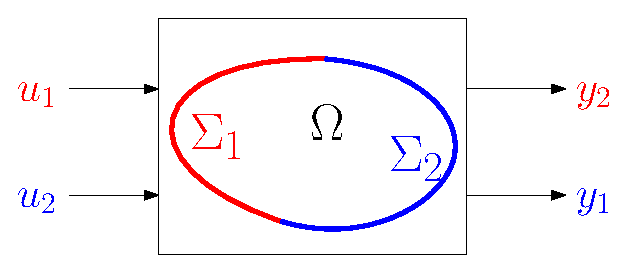
\includegraphics[width=6cm]{bound_part.eps}
	\end{figure}
	
	\vspace{1cm}
	This can be achieved by weak imposition of the boundary conditions via the Hellinger-Reissner variational principle \footfullcite{thoma2021explicit}.
	
	

\end{frame}

\begin{frame}{Weak and strong imposition}
	There is no general consensus upon which approach performs better:
	
	\begin{itemize}
		\item  "For boundary layer solutions of the incompressible Navier-Stokes eqs, it is found that \textbf{weakly enforced conditions are superior to strongly enforced ones}."\footfullcite{bazilevs2007weak}
		\item "Numerical experiments also show that \textbf{subtle effects close to solid walls are more efficiently captured with strong boundary condition imposition} methods rather than weak (less dofs. required)."\footfullcite{eriksson2022}
	\end{itemize}

Strong impositon of BCs. is cumbersome for $H^2$ conforming elements and penalty methods are preferred\footfullcite{kirby2019mapped}.  
\end{frame}

\section{Abstract framework and examples}
	
\begin{frame}{Notation}
	$\Omega\subset \bbR^d$ (bounded connected) with $d = \{1,2,3\}$  and  $\partial\Omega=  \overline{\Sigma}_1 \cup \overline{\Sigma}_2$ and $\Sigma_1 \cap \Sigma_2 = \emptyset$. Each $\Sigma_i$ associated to a specific BC, captured by the trace operator~$\gamma_i$.
	
	Let $\bbA, \; \bbB$ be vector spaces and $L$ an unbounded operator 
	\begin{equation*}
		L: L^2(\Omega, \bbA) \rightarrow L^2(\Omega, \bbB), \qquad
		D(L) = \{u \in L^2(\Omega, \bbA)|\; L u \in L^2(\Omega, \bbB)\}.
	\end{equation*} 
	We denote by $L^\dag$, with domain
	\begin{equation*}
		D(L^\dag) = \{u \in L^2(\Omega, \bbB)|\; L^\dag u \in L^2(\Omega, \bbA)\},
	\end{equation*}
	a formal adjoint operator of $L$ with respect to the $\gamma_i$ operators, \textit{i.e.} 
	$$
	\inner[\Omega]{L e_1}{e_2} = \inner[\Omega]{e_1}{L^\dag e_2}, \qquad \forall 
	e_i \in \ker \left( \gamma_i^{\Sigma_i} \right), \qquad i \in \{1,2\}
	$$
	where $\gamma_i^{\Sigma_i}$ is the restriction of the operator $\gamma_i$ to $\Sigma_i$ and $\inner[\Omega]{\cdot}{\cdot}$ is the $L^2$ inner product for a suitable vector space ($\bbA$ or $\bbB$).
	
\end{frame}	

\begin{frame}{Main assumption}
\begin{assumption}[Abstract integration by parts]\label{Assumption-IBP}
	The operators $L$ and $L^\dag$ are assumed to satisfy the integration by parts formula
	\begin{equation*}\label{eq:intbyparts}
		\inner[L^2(\Omega, \bbB)]{L e_1}{e_2} - \inner[L^2(\Omega, \bbA)]{e_1}{L^\dag e_2} = \dualpr[V_\partial, V_\partial']{\gamma_1 e_1}{\gamma_2 e_2},
	\end{equation*}
	where $\dualpr[V_\partial, V_\partial']{\cdot}{\cdot}$ is the duality product between the boundary space $V_\partial$ and its dual $V_\partial'$.
\end{assumption}

\begin{tcolorbox}[nobeforeafter, colframe=theme,title=Example: {$L=\grad: L^2(\Omega) \rightarrow L^2(\Omega, \bbR^d), \; D(\grad)=H^1(\Omega)$}]%%
	Operator $\gamma_1$ is the Dirichlet trace, $\gamma_2$ is the normal trace 
	\begin{equation*}
		\gamma_1 u= u\vert_{\partial\Omega}, \qquad \gamma_2 \bm{v}= \bm{v} \cdot \bm{n}\vert_{\partial\Omega}.
	\end{equation*}
$L^\dag = -\div$ with domain $H^{\div}(\Omega)$. The assumption is simply the Green's formula
\begin{equation*}
	\int_\Omega \grad u \cdot \bm{v} = - \int_\Omega u \div \bm{v} + \dualpr[H^{\frac{1}{2}}(\partial\Omega), H^{-\frac{1}{2}}(\partial\Omega)]{u}{\bm{v} \cdot \bm{n}}.
\end{equation*}
\end{tcolorbox} 

\end{frame}

\begin{frame}{Boundary control operator and compatibility conditions}
	Let $\mathcal{L}(X, Y)$ be the set of bounded linear operators from $X$ to $Y$.
	The boundary control operator is given by
\begin{equation*}
	G_u = \begin{bmatrix}
		\gamma_1^{\Sigma_1} & 0 \\
		0 & \gamma_2^{\Sigma_2}
	\end{bmatrix} \in \mathcal{L}(D(L) \times D(L^\dag), \mathcal{U}_1 \times \mathcal{U}_2), \qquad \mathcal{U}_i \text{ control spaces.}
\end{equation*}


Compatibility relations at the interface(s) $\overline{\Sigma_1} \cap \overline{\Sigma_2}$ must be fulfilled by $u_i \in \mathcal{U}_i$.\\
 If the boundary control system is well-posed, then $\mathcal{U}_i \subset {\rm Range}( \gamma_i^{\Sigma_i} )$ and it holds
\begin{equation*}
	\begin{aligned}
		\dualpr[V_\partial,V_\partial']{\gamma_1 e_1}{\gamma_2 e_2} =& \dualpr[V_{\partial, 1},V_{\partial, 1}']{\gamma_1^{\Sigma_1} e_1}{\gamma_2^{\Sigma_1} e_2} + \dualpr[V_{\partial, 2},V_{\partial, 2}']{\gamma_1^{\Sigma_2} e_1}{\gamma_2^{\Sigma_2} e_2}, \\
		=& \dualpr[V_{\partial, 1},V_{\partial, 1}']{u_1}{y_1} + \dualpr[V_{\partial, 2},V_{\partial, 2}']{y_2}{u_2}, \\
		=& \dualpr[\mathcal{U}_1, \mathcal{Y}_1]{u_1}{y_1} + \dualpr[\mathcal{Y}_2, \mathcal{U}_2]{y_2}{u_2}.
	\end{aligned}
\end{equation*}
The input and output functional spaces are defined accordingly to the splitting
\begin{equation*}
	\begin{aligned}
		\mathcal{U}_1 \subset V_{\partial, 1} := {\rm Range}( \gamma_1^{\Sigma_1} ), \\
		\mathcal{U}_2 \subset V_{\partial, 2}' := {\rm Range}( \gamma_2^{\Sigma_2} ),
	\end{aligned} \qquad
	\begin{aligned}
		\mathcal{Y}_1 \supset V_{\partial, 1}', \\
		\mathcal{Y}_2 \supset V_{\partial, 2}.
	\end{aligned}
\end{equation*}

\end{frame}

\begin{frame}{Second assumption}
	\begin{assumption}[Compatibility conditions]
		The compatibility conditions at $\overline{\Sigma_1} \cap \overline{\Sigma_2}$ are fulfilled. \\
		Consequently we do not discriminate between boundary spaces 
		\begin{equation*}
			\begin{aligned}
				\dualpr[\Sigma_1]{\cdot}{\cdot} &:= \dualpr[\mathcal{U}_1,\mathcal{Y}_1]{\cdot}{\cdot} = \dualpr[V_{\partial,1},V_{\partial,1}']{\cdot}{\cdot}, \\
				\dualpr[\Sigma_2]{\cdot}{\cdot} &:= \dualpr[\mathcal{Y}_2,\mathcal{U}_2]{\cdot}{\cdot}=  \dualpr[V_{\partial,2},V_{\partial,2}']{\cdot}{\cdot}, \\
				\dualpr[\partial\Omega]{\cdot}{\cdot} &:= \dualpr[V_\partial,V_\partial']{\cdot}{\cdot}
			\end{aligned}
		\end{equation*}
	Hence, the abstract integration by parts formula of Assumption~\ref{Assumption-IBP} can be  rewritten as
	\begin{equation}\label{eq:intbyparts-for-mixed}
		\inner[\Omega]{L e_1}{e_2} - \dualpr[\Sigma_1]{\gamma_1 e_1}{\gamma_2 e_2} 
		= \inner[\Omega]{e_1}{L^\dag e_2} + \dualpr[\Sigma_2]{\gamma_1 e_1}{\gamma_2 e_2}.
	\end{equation}
	\end{assumption}

\end{frame}

\begin{frame}{Abstract linear hyperbolic port-Hamiltonian systems}
	We focus on linear pH systems of the form (co-energy formulation)
\begin{equation*}
	\begin{aligned}
		\begin{bmatrix}
			Q_1 & 0 \\
			0 & Q_2
		\end{bmatrix}\diffp{}{t}\begin{pmatrix}
			e_1 \\ e_2
		\end{pmatrix} = 
		\begin{bmatrix}
			0 & -L^\dag \\
			L & 0 \\
		\end{bmatrix}\begin{pmatrix}
			e_1 \\ e_2
		\end{pmatrix}, \\
		H = \frac{1}{2}\inner[\Omega]{e_1}{Q_1 e_1} + \frac{1}{2}\inner[\Omega]{e_2}{Q_2 e_2}.
	\end{aligned}
\end{equation*}
The operators $Q_1, \; Q_2$ are bounded, symmetric and uniformly positive. \\
The boundary inputs and outputs are
\begin{equation*}
	\begin{pmatrix}
		u_1 \\ u_2
	\end{pmatrix} = \begin{bmatrix}
	\gamma_1^{\Sigma_1} & 0 \\
	0 & \gamma_2^{\Sigma_2}
\end{bmatrix} = G_u
	\begin{pmatrix}
		e_1 \\ e_2
	\end{pmatrix}, \qquad 	\begin{pmatrix}
	y_1 \\ y_2
\end{pmatrix} = 
\begin{bmatrix}
0 & \gamma_2^{\Sigma_1} \\
\gamma_1^{\Sigma_2} & 0
\end{bmatrix} 
\begin{pmatrix}
e_1 \\ e_2
\end{pmatrix} = G_y
\begin{pmatrix}
e_1 \\ e_2
\end{pmatrix},
\end{equation*}
where $G_y \in \mathcal{L}(D(L) \times D(L^\dag), \mathcal{Y}_1 \times \mathcal{Y}_2)$. Thanks to Eq. \eqref{eq:intbyparts-for-mixed}
\begin{equation*}
	\dot{H} = \dualpr[\Sigma_1]{u_1}{y_1} + \dualpr[\Sigma_2]{y_2}{u_2}.
\end{equation*}
\end{frame}



\begin{frame}{The wave equation}
	\begin{equation*}
		\begin{bmatrix}
			\kappa^{-1} & 0 \\
			0 & \rho
		\end{bmatrix}\diffp{}{t}\begin{pmatrix}
			p \\ \bm{u}
		\end{pmatrix} = 
		\begin{bmatrix}
			0 & \div \\
			\grad & 0 \\
		\end{bmatrix}\begin{pmatrix}
			p \\ \bm{u}
		\end{pmatrix},  \qquad \Omega \subset \bbR^d
	\end{equation*}
Unknowns:
\begin{itemize}
\item the pressure scalar field $p : \Omega \times (0, t_{\mathrm{end}}) \rightarrow \bbR$;
\item the velocity vector field $\bm{u} : \Omega \times (0, t_{\mathrm{end}}) \rightarrow \bbR^d$.
\end{itemize}
Parameters:
\begin{itemize}
\item the bulk modulus $\kappa: \Omega \rightarrow \bbR_+$ \\
\item the mass density $\rho: \Omega \rightarrow \bbR_+$.
\end{itemize}
\end{frame}

\begin{frame}{Linear Elastodynamics}
	\begin{equation*}
		\begin{bmatrix}
			\rho & 0 \\
			0 & \bm{\mathcal{C}}
		\end{bmatrix}\diffp{}{t}\begin{pmatrix}
			\bm{u} \\ \bm{\Sigma} 
		\end{pmatrix} = 
		\begin{bmatrix}
			0 & \Div \\
			\Grad & 0 \\
		\end{bmatrix}\begin{pmatrix}
			\bm{u} \\ \bm{\Sigma}
		\end{pmatrix}, \qquad \Omega \subset \bbR^d
	\end{equation*}
where $\Grad\bm{u}=\frac{1}{2}(\nabla \bm{u} + \nabla^\top \bm{u})$ and $\Div \bm{\Sigma}= \sum_{i=1}^d \partial_{x_i} [\bm\Sigma]_{ij}$.\\

	Unknowns 
	\begin{itemize}
		\item the velocity field $\bm{u} : \Omega \times (0, t_{\mathrm{end}}) \rightarrow \bbR^d$;
		\item the symmetric stress tensor $\bm{\Sigma} : \Omega \times (0, t_{\mathrm{end}}) \rightarrow \bbR^{d\times d}_{\text{sym}}$.
	\end{itemize}
	 $\bm{\mathcal{C}}: \Omega \rightarrow \mathcal{L}(\bbR^{d\times d}_{\text{sym}})$ is the compliance fourth order tensor (positive and symmetric). 
	 
	\begin{equation*}
		\inner[\Omega]{\Grad \bm{u}}{\Sigma} + \inner[\Omega]{\bm{u}}{\Div \Sigma} = \dualpr[\partial\Omega]{\bm{u}}{\bm{\Sigma} \cdot \bm{n}}.
	\end{equation*}
	The boundary duality product involve the spaces
	\begin{equation*}
			V_\partial = H^{1/2}(\partial\Omega, \bbR^d), \qquad  V_\partial^{'} = H^{-1/2}(\partial\Omega, \bbR^d).
	\end{equation*}
\end{frame}


\begin{frame}{The Maxwell equations}
	\begin{equation*}
		\begin{bmatrix}
			\varepsilon & 0 \\
			0 & \mu
		\end{bmatrix}\diffp{}{t}\begin{pmatrix}
			\bm{E} \\ \bm{H} 
		\end{pmatrix} = 
		\begin{bmatrix}
			0 & \curl \\
			-\curl & 0 \\
		\end{bmatrix}\begin{pmatrix}
			\bm{E} \\ \bm{H}
		\end{pmatrix},  \qquad \Omega \subset \bbR^3
	\end{equation*}
	Unknowns:
\begin{itemize}
	\item the electric field $\bm{E} : \Omega \times (0, t_{\mathrm{end}}) \rightarrow \bbR^3$;
	\item the magnetic field $\bm{H} : \Omega \times (0, t_{\mathrm{end}}) \rightarrow \bbR^3$.
\end{itemize}
Parameters:
\begin{itemize}
	\item the electric permittivity $\varepsilon: \Omega \rightarrow \bbR^{3\times 3}_{\text{sym}}>0$;
	\item the magnetic permeability $\mu:\Omega \rightarrow \bbR^{3\times 3}_{\text{sym}} > 0$.
\end{itemize}
	\begin{equation*}
		\inner[\Omega]{-\curl \bm{E}}{\bm{H}} + \inner[\Omega]{\bm{E}}{\curl \bm{H}} = \dualpr[\partial\Omega]{\bm{E} \times \bm{n}}{\bm{n} \times (\bm{H} \times \bm{n})}.
	\end{equation*}

	The trace space $V_\partial$ then corresponds to
	\begin{equation*}
		V_\partial = \{\bm{f} \in (H^{-1/2}(\partial\Omega))^3 \vert \; \exists \bm{\xi} \in H^{\curl} \text{ s.t. } \bm{\xi}\times \bm{n}\vert_{\partial\Omega} = \bm{f}\}.
	\end{equation*}
	$V_\partial'$ corresponds to the topological dual (whose characterization is really involved). 
\end{frame}

\section{Generalized Hellinger-Reissner principle and associated discretization}

\begin{frame}{Weak formulation}
	Consider a weak formulation of the dynamics
	\begin{equation*}
		\begin{aligned}
			\inner[\Omega]{v_1}{Q_1 \partial_t e_1} &= -\inner[\Omega]{v_1}{L^\dag e_2}, \\
			\inner[\Omega]{v_2}{Q_2 \partial_t e_2} &= +\inner[\Omega]{v_2}{L e_1}.
		\end{aligned}
	\end{equation*}
	A completely analogous formulation is obtained by summing a zero contribution
	\begin{equation*}
		u_1 - \gamma_1^{\Sigma_1} e_1 = 0, \qquad u_2 - \gamma_2^{\Sigma_2} e_2 =0.
	\end{equation*}
	Taking the duality product of these expressions with test functions $v_1,  \; v_2$ leads to a modified weak formulation
	\begin{equation*}
		\begin{aligned}
			\inner[\Omega]{v_1}{Q_1 \partial_t e_1} &= -\inner[\Omega]{v_1}{L^\dag e_2} + \dualpr[\Sigma_2]{\gamma_1 v_1}{u_2 - \gamma_2 e_2}, \\
			\inner[\Omega]{v_2}{Q_2 \partial_t e_2} &= +\inner[\Omega]{v_2}{L e_1} + \dualpr[\Sigma_1]{u_1 - \gamma_1 e_1}{\gamma_2 v_2}.
		\end{aligned}
	\end{equation*}
\end{frame}

\begin{frame}{Integration by parts of the $L^\dag$ operator}
	Using \eqref{eq:intbyparts-for-mixed}, if $L^\dag$ is integrated by parts the first weak formulation is obtained: \\
	find $e_1 \in D(L), \; e_2 \in D(L^\dag)$ such that
	\begin{equation*}
		\begin{aligned}
			\inner[\Omega]{v_1}{Q_1 \partial_t e_1} = &-\inner[\Omega]{L v_1}{e_2} + \dualpr[\Sigma_1]{\gamma_1 v_1}{\gamma_2 e_2} + \dualpr[\Sigma_2]{\gamma_1 v_1}{u_2}, \\
			\inner[\Omega]{v_2}{Q_2 \partial_t e_2} = &+\inner[\Omega]{v_2}{L e_1} - \dualpr[\Sigma_1]{\gamma_1 e_1}{\gamma_2 v_2} + \dualpr[\Sigma_1]{u_1}{\gamma_2 v_2}.
		\end{aligned} \qquad
		\begin{aligned}
		\forall v_1 \in D(L), \\
	    \forall v_2 \in D(L^\dag).
		\end{aligned}
	\end{equation*}
	The test functions do include boundary conditions. \\
	Notice that, the bilinear form 
	\begin{equation*}
		\begin{aligned}
			j_{L, \Sigma_1}( (v_1, v_2), (e_1, e_2)) = &-\inner[\Omega]{L v_1}{e_2} + \dualpr[\Sigma_1]{\gamma_1 v_1}{\gamma_2 e_2} \\
			&+\inner[\Omega]{v_2}{L e_1} - \dualpr[\Sigma_1]{\gamma_1 e_1}{\gamma_2 v_2},
		\end{aligned}
	\end{equation*}
	is  skew symmetric. 
\end{frame}

\begin{frame}{Integration by parts of the $L$ operator}
	Using \eqref{eq:intbyparts-for-mixed}, if $L$ is integrated by parts the second weak formulation is obtained: \\
	find $e_1 \in D(L), \; e_2 \in D(L^\dag)$ such that
	\begin{equation*}
	\begin{aligned}
		\inner[\Omega]{v_1}{Q_1 \partial_t e_1} = &-\inner[\Omega]{v_1}{L^\dag e_2} - \dualpr[\Sigma_2]{\gamma_1 v_1}{\gamma_2 e_2} + \dualpr[\Sigma_2]{\gamma_1 v_1}{u_2}, \\
		\inner[\Omega]{v_2}{Q_2 \partial_t e_2} = &+\inner[\Omega]{L^\dag v_2}{e_1} + \dualpr[\Sigma_2]{\gamma_1 e_1}{\gamma_2 v_2} + \dualpr[\Sigma_1]{u_1}{\gamma_2 v_2},
	\end{aligned} \qquad
	\begin{aligned}
	\forall v_1 \in D(L), \\
	\forall v_2 \in D(L^\dag).
	\end{aligned}
	\end{equation*}
	The bilinear form 
	\begin{equation*}
		\begin{aligned}
			j_{L^\dag,\Sigma_2}((v_1, v_2), (e_1, e_2)) = &-\inner[\Omega]{v_1}{L^\dag e_2} - \dualpr[\Sigma_2]{\gamma_1 v_1}{\gamma_2 e_2}  \\
			&+\inner[\Omega]{L^\dag v_2}{e_1} + \dualpr[\Sigma_2]{\gamma_1 e_1}{\gamma_2 v_2},
		\end{aligned}
	\end{equation*}
	is skew symmetric. 
\end{frame}

\begin{frame}{Properties of the weak formulations}
	\begin{proposition}[Equivalence of the formulations]\label{pr:equivalence}
		Since $v_1,\ e_1 \in D(L)$ and $v_2,\ e_2 \in D(L^\dag)$, by using the integration by parts \eqref{eq:intbyparts-for-mixed}  on the appropriate line of the bilinear forms $j_{L,\Sigma_1}$ or $j_{L^\dag,\Sigma_2}$, it holds $j_{L,\Sigma_1} = j_{L^\dag,\Sigma_2}$. 
	\end{proposition}

\begin{proposition}[Connection with Lagrange multiplier method]
If the BC on $\Sigma_1$ is imposed via a Lagrange multiplier. then $\lambda$ is the multiplier associated to  the constraint $u_1 - \gamma_1^{\Sigma_1} e_1 = 0$. Using 
Eq.~\eqref{eq:intbyparts} an the extended system in weak form is obtained: find $e_1 \in D(L), \; e_2 \in D(L^\dag), \; \lambda \in \gamma_2^{\Sigma_1}\left(D(L^\dag)\right)$ such that
\begin{equation*}
	\begin{aligned}
		\inner[\Omega]{v_1}{Q_1 \partial_t e_1} &= -\inner[\Omega]{L v_1}{e_2}
		+\dualpr[\Sigma_1]{\gamma_1 v_1}{\lambda}
		+\dualpr[\Sigma_2]{\gamma_1 v_1}{u_2}, \\
		\inner[\Omega]{v_2}{Q_2 \partial_t e_2} &= +\inner[\Omega]{v_2}{L e_1}, \\
		0 &= \dualpr[\Sigma_1]{u_1 - \gamma_1 e_1}{v_\lambda},
	\end{aligned}
\end{equation*}
Since $\lambda = y_1 := \gamma_2^{\Sigma_1} e_2$, if $v_\lambda = \gamma_2 v_2$ and substituting the third line in the second one obtains to previous $L$ weak formulation (and analogously for $L^\dag$).

\end{proposition}

\end{frame}

\begin{frame}{First finite dimensional systems}
Galerkin expansion for test functions, states and control inputs ($\bm{x} \in \Omega, \; \bm{s}_i \in \Sigma_i$)
\begin{equation*}
	\begin{aligned}
		v_i = \sum_{m=1}^{N_i} \phi_i^m(\bm{x}) v_i^m, \qquad e_i = \sum_{m=1}^{N_i} \phi_i^m(\bm{x}) e_i^m(t), \qquad u_i = \sum_{m=1}^{N_{i, \partial}} \psi_i^m(\bm{s}_i) u_i^m(t),
	\end{aligned}
\end{equation*}
The following finite-dimensional system is obtained from the first weak formulation 
\begin{equation*}
	\begin{bmatrix}
		\mathbf{M}_1 & \mathbf{0} \\
		\mathbf{0} & \mathbf{M}_2
	\end{bmatrix} \begin{pmatrix}
		\dot{\mathbf{e}}_1 \\
		\dot{\mathbf{e}}_2
	\end{pmatrix} = \begin{bmatrix}
		\mathbf{0} & -\mathbf{K}_{L}^\top \\
		\mathbf{K}_{L} & \mathbf{0}
	\end{bmatrix} \begin{pmatrix}
		\mathbf{e}_1 \\
		\mathbf{e}_2
	\end{pmatrix} + 
	\begin{bmatrix}
		\mathbf{0} & \mathbf{B}_{2} \\
		\mathbf{B}_{1} & \mathbf{0}
	\end{bmatrix} \begin{pmatrix}
		\mathbf{u}_1 \\
		\mathbf{u}_2
	\end{pmatrix},
\end{equation*}
\begin{equation*}
	[\mathbf{M}_i]_{mn} = \inner[\Omega]{\phi_i^m}{Q_i \phi_i^n}, \qquad 	[\mathbf{K}_{L}]_{mn} = \inner[\Omega]{\phi_2^m}{L \phi_1^n} - \dualpr[\Sigma_1]{\gamma_1 \phi_1^n}{\gamma_2 \phi_2^m}.
\end{equation*}
The control matrices are computed via
\begin{equation*}
	[\mathbf{B}_{1}]_{mn} = \dualpr[\Sigma_1]{\psi_1^n}{\gamma_2\phi_2^m}, \qquad [\mathbf{B}_{2}]_{mn} = \dualpr[\Sigma_2]{\gamma_1\phi_1^m}{\psi_2^n}.
\end{equation*}

\end{frame}

\begin{frame}{Second finite dimensional systems}
	Symmetrically, starting from the second formulation, the following system is readily obtained
	\begin{equation*}
		\begin{bmatrix}
			\mathbf{M}_1 & \mathbf{0} \\
			\mathbf{0} & \mathbf{M}_2
		\end{bmatrix} \begin{pmatrix}
			\dot{\mathbf{e}}_1 \\
			\dot{\mathbf{e}}_2
		\end{pmatrix} = \begin{bmatrix}
			\mathbf{0} & -\mathbf{K}_{L^\dag} \\
			\mathbf{K}_{L^\dag}^\top & \mathbf{0}
		\end{bmatrix} \begin{pmatrix}
			\mathbf{e}_1 \\
			\mathbf{e}_2
		\end{pmatrix} + 
		\begin{bmatrix}
			\mathbf{0} & \mathbf{B}_{2} \\
			\mathbf{B}_{1} & \mathbf{0}
		\end{bmatrix} \begin{pmatrix}
			\mathbf{u}_1 \\
			\mathbf{u}_2
		\end{pmatrix},
	\end{equation*}
	where the differentiation matrix $\mathbf{D}_{L^\dag}$ now reads
	\begin{equation*}
		[\mathbf{K}_{L^\dag}]_{mn} = \inner[\Omega]{\phi_1^m}{L^\dag \phi_2^n} + \dualpr[\Sigma_2]{\gamma_1 \phi_1^m}{\gamma_2 \phi_2^n}.
	\end{equation*}
	
	\begin{proposition}[Algebraic Stokes theorem]
		From the equivalence of the formulation, for conforming discrete spaces 
		\begin{equation*}
			\begin{aligned}
				\mathrm{span}(\phi_1^1, \dots, \phi_1^{N_1}) &= V_L \subset D(L), \\
				\mathrm{span}(\phi_2^1, \dots, \phi_2^{N_2}) &= V_{L^\dag} \subset D(L^\dag),
			\end{aligned}
		\end{equation*}
		 the Stokes theorem leads to the algebraic relation $\mathbf{K}_L^\top = \mathbf{K}_{L^\dag}$.
	\end{proposition}
	
\end{frame}


\section{Numerical experiment}

\begin{frame}{Eigenproblem for the 2D wave equation with unitary parameters}
	Domain data:
	\begin{equation*}
		\Omega = \{(x,y) \in [0, \pi] \times [0, \pi]\},\qquad 
		\Sigma_1= \{x=0 \cup x=\pi\}, \qquad \Sigma_2 = \{y=0 \cup y=\pi\}.
	\end{equation*}
	Analytical eigenvalues take the form
	\begin{equation*}
		\begin{aligned}
			\lambda_{\mathrm{ex}}=\pm j \omega_{\mathrm{ex}}, \qquad 	\omega_{\mathrm{ex}} = \sqrt{n^2 + m^2},\qquad  \forall n \in \mathbb{N}_{0}, \; \forall m \in \mathbb{N}_{>0}, \qquad j=\sqrt{-1}
		\end{aligned}
	\end{equation*}
The $\grad$ formulation is employed and 
\begin{equation*}
		p_h \in \mathrm{CG}_r, \quad \bm{u}_h \in \mathrm{RT}_r.
\end{equation*}
 For the discretization 5 triangular elements per side are used.

 
\begin{remark}
	The weak formulations are more restrictive for the choice of  finite elements,  since both spaces need to be conforming. FE spaces will not form a de Rham subcomplex in general.
\end{remark}

\end{frame}

\begin{frame}{Results}
	
	Eigensolver: Krylov-Schur solver from SLEPc with shift and invert spectral transform.
	
	\begin{figure}
		\centering
		\subfloat[][Weak imposition]{%
			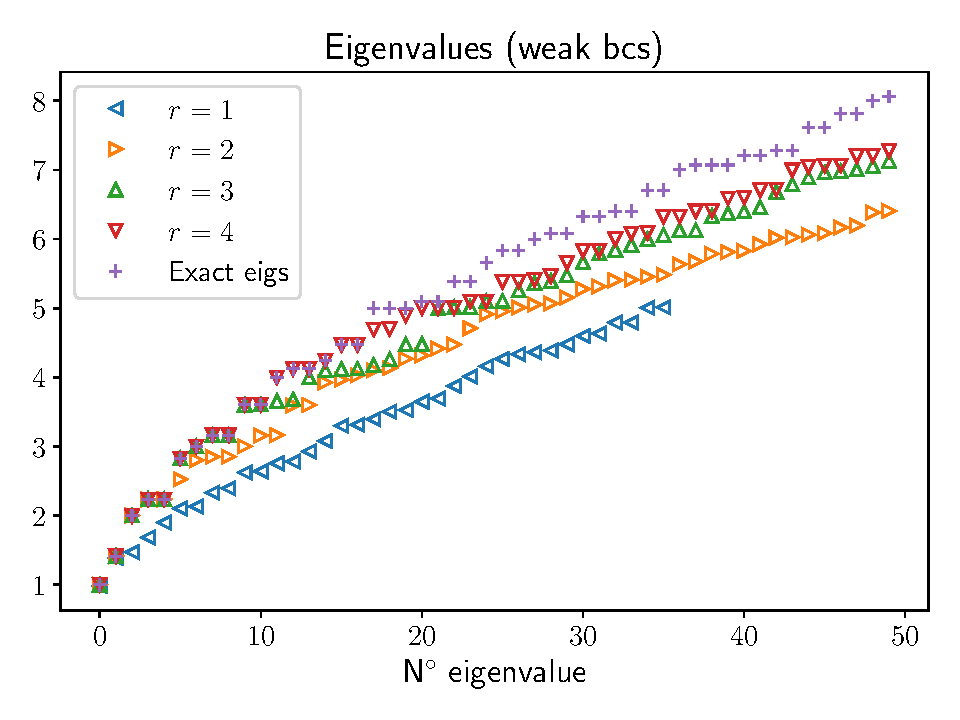
\includegraphics[width=.45\textwidth]{Eigs_weak.pdf}}%
		\subfloat[][Strong imposition]{%
			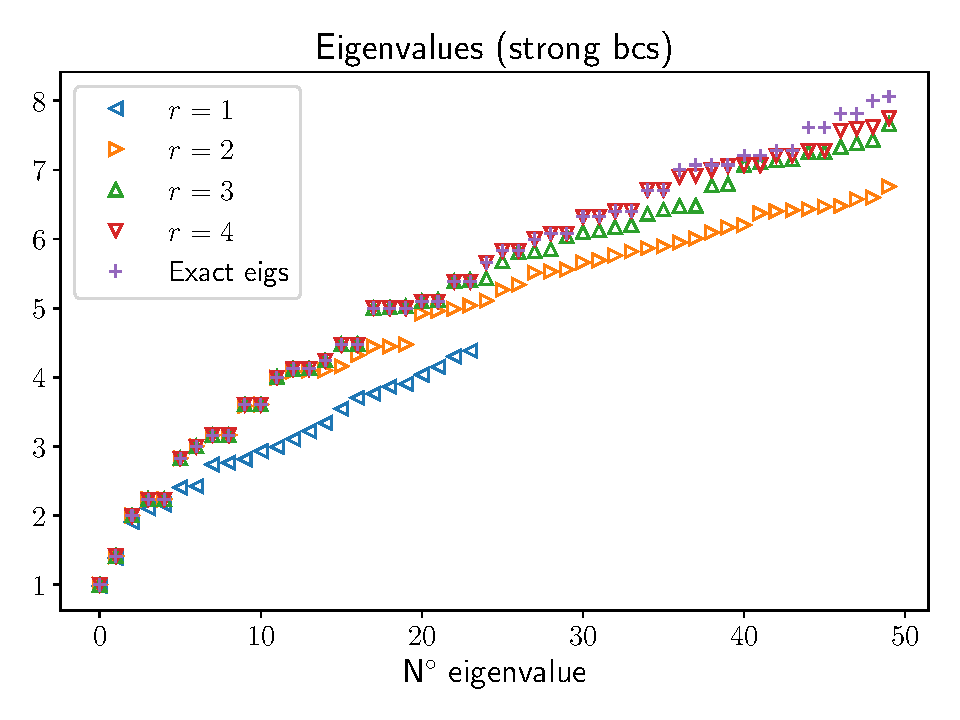
\includegraphics[width=.45\textwidth]{Eigs_strong.pdf}}%
		\caption*{Eigenvalues for different polynomial orders}%
	\end{figure}
	

\end{frame}

\begin{frame}{Conclusion}
	This approach allows avoiding the need to deal with differential algebraic systems but:
	\begin{itemize}
		\item the choice of the finite elements is restricted to more regular elements, that in general will not satisfy de Rham subcomplex property.
		\item The results for the considered
		test case show that the approach performs rather poorly
		compared to the standard strong imposition.
	\end{itemize}
\end{frame}

\begin{frame}{Bibliography}
	%\nocite{*}
	\printbibliography
\end{frame}

	\appendix
	
	
	
	
\end{document}